% !TEX TS-program = pdflatex
% !TEX encoding = UTF-8 Unicode
% !TEX ROOT = ../../main.tex

\section{Zoo}

Direkter Nachbar der Jugendherberge ist der Zoo Heidelberg. Er wurde bereits 1933 durch den Chemienobelpreisträger Carl Bosch und den Ornithologen Otto Fehringer auf dem Gelände eines ehemaligen Friedhofs gegründet. Mit einer Fläche von ca. 12 ha und etwa 500.000 Besuchern pro Jahr ist er ein eher kleiner Zoo, hat aber dennoch einiges zu bieten.

Der Zoo hält etwa 163 Tierarten, darunter Publikumslieblinge wie Flachlandgorillas, Schimpansen, Berberlöwen und Sumatratiger. Aber auch eher unbekannte Tierarten, von der Asiatischen Goldkatze bis zum Waldrapp, können im Zoo beobachtet werden.

Dabei beteiligt sich der Zoo erfolgreich an Artenschutzmaßnahmen, z.\,B.\,an 39 Europäischen Erhaltungszuchtprogrammen, und ist -- auch mithilfe der Zooschule -- eine wichtige Stätte der Umweltbildung.

Eine unbedingt sehenswerte Besonderheit im Zoo Heidelberg ist die erste Jungbullengruppe von Asiatischen Elefanten in Deutschland: Die Elefantenkühe und ihre Jungtiere leben in der Natur in Herden zusammen, erwachsene Bullen stoßen nur zur Paarung dazu. Junge männliche Elefanten werden im Alter von einigen Jahren aus ihren Herden ausgestoßen und schließen sich dann kleinen Jungbullenverbänden an, bis sie selbst paarungsbereit sind. Diese natürliche Sozialstruktur kann durch die innovative Haltung im Zoo Heidelberg auch heranwachsenden Elefanten aus europäischen Zoos geboten werden, die einige Jahre in Heidelberg verbringen, bis sie als erwachsener Bulle in einen anderen Zoo umziehen. 

Auch die Parkanlage des Zoos ist sehr schön und lädt zum Spazierengehen ein, man sollte sich allerdings darauf einstellen, dass gerade mitten im Zoo eine große Baustelle ist, weil ein neues Gehege für die Heidelberger Löwen errichtet wird.

Der Eintritt kostet für Studierende 8,50€. Gäste der Jugendherberge können Karten auch direkt dort kaufen. Im Preis enthalten ist der Eintritt in die \glqq Meere und Ozeane\grqq{}  Sonderausstellung im ExploHeidelberg.

\begin{figure}[h]
\captionsetup[subfigure]{labelformat=empty} 
\centering
\begin{subfigure}{0.5\textwidth}
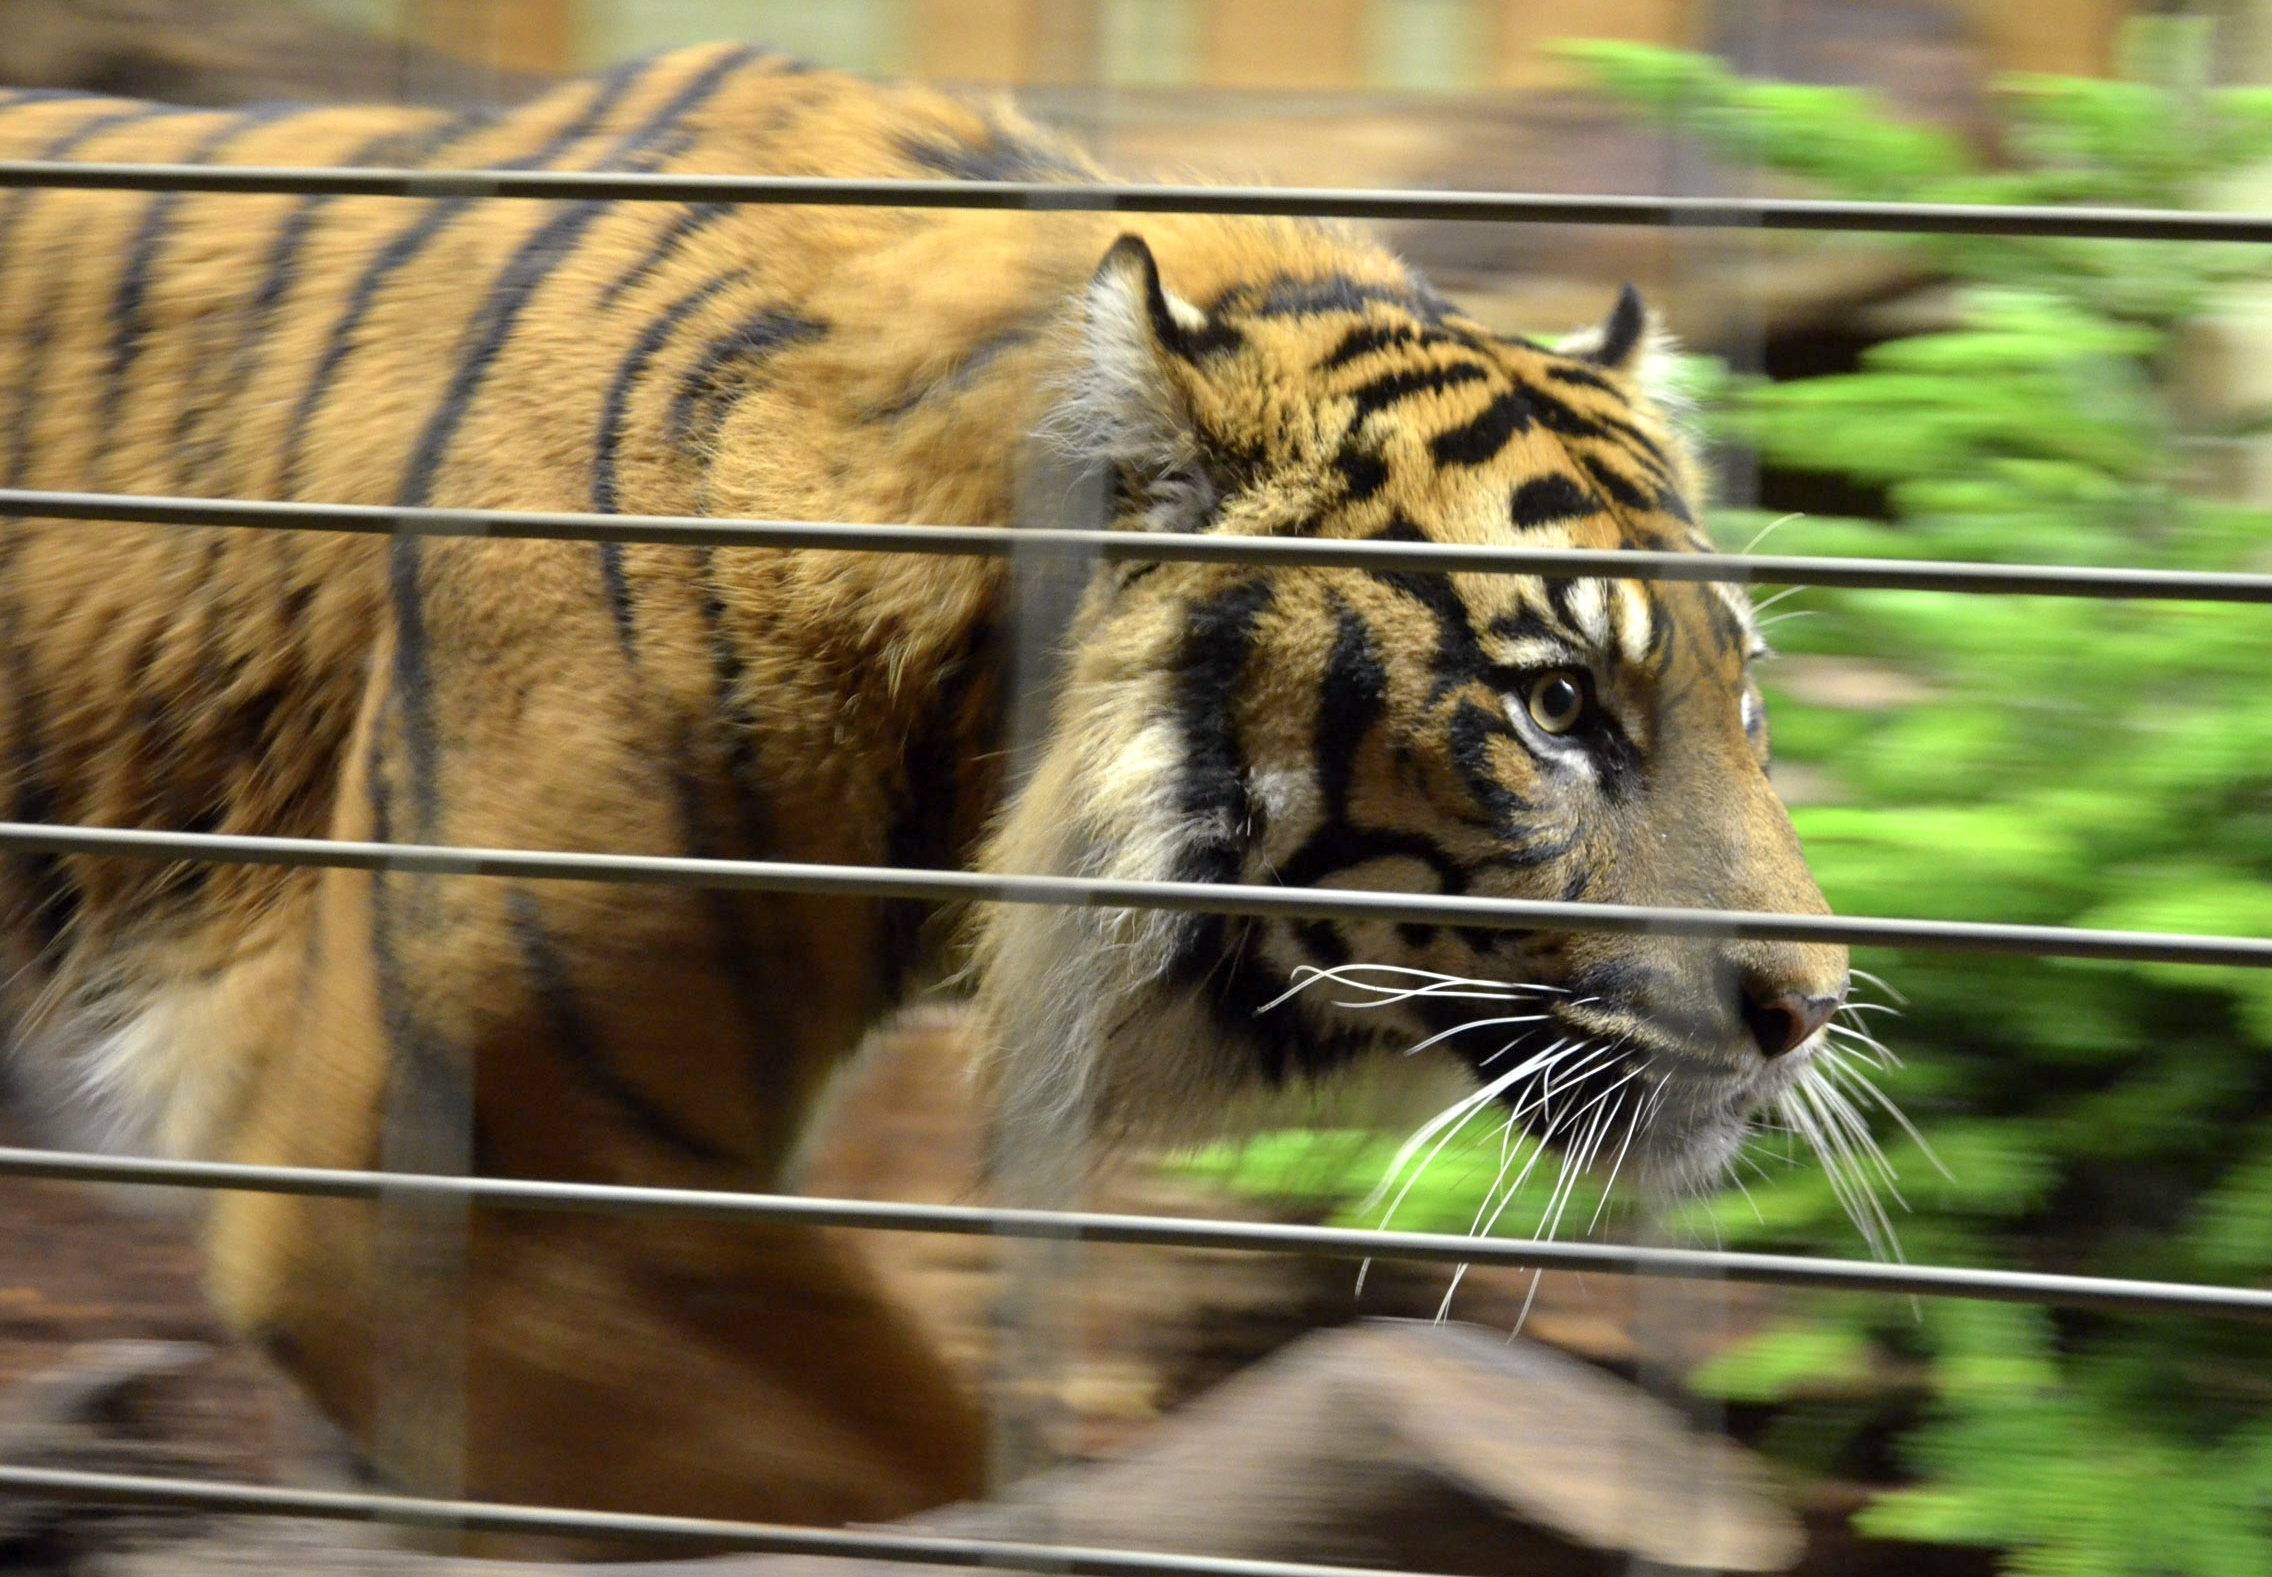
\includegraphics[width=0.9\linewidth]{tigga.jpg} 
\end{subfigure}
\begin{subfigure}{0.3\textwidth}
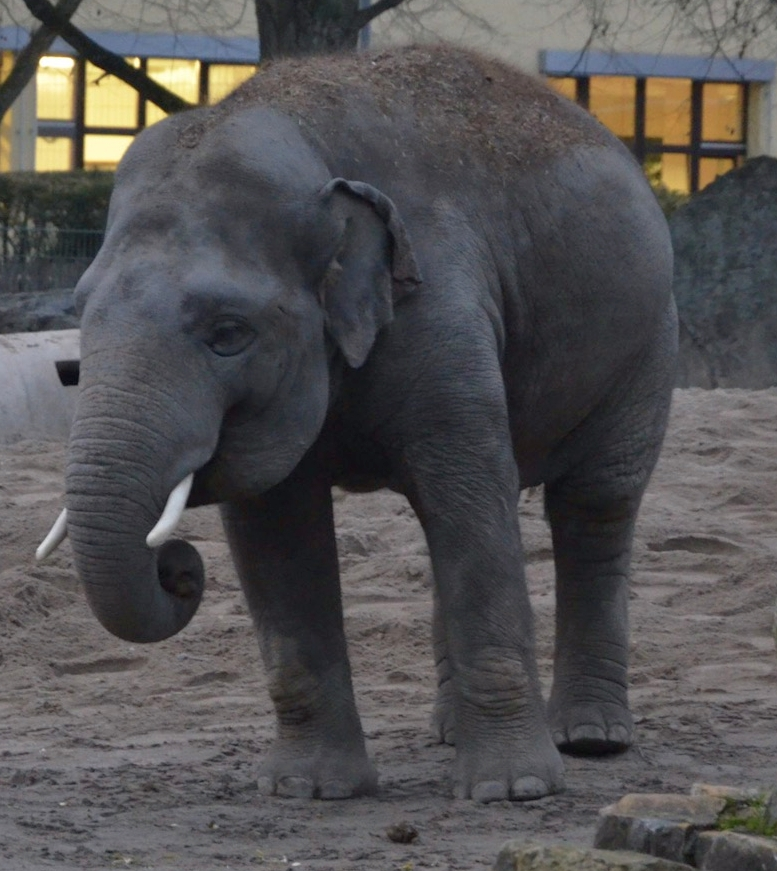
\includegraphics[width=0.9\linewidth]{eli.jpg}
\end{subfigure}
\end{figure}